\subsection{Незамкнутая трофическая цепь}
    \subsubsection{Равновесные состояния}
        Поскольку единственное положительное слагаемое, которое описывает вносимое количество биомассы, в каждой строке зависит от количества биомассы предыдущего вида, то можно сделать вывод, что если в каком-то состоянии равновесия будет вид с нулевой биомассой, то и все последующие виды так же окажутся вымершими.

        Поэтому в системе (\ref{flow}) при \(Q > 0\) могут существовать \( n \) равновесных состояний типа \(\left[ N_0, N_1, \ldots, N_q, 0, \ldots, 0 \right]\), которые можно определить из уравнений
        \begin{equation} \label{flow_stationary_equations}
            \frac{dN}{dt} = 0 \Rightarrow
            \left\lbrace\begin{split}
                & N_1 = \frac{Q}{\alpha_0 N_0}, \\
                & \alpha_i N_{i+1} = k_i \alpha_{i-1} N_{i-1} - m_i, \quad i=\overline{1,q}                
            \end{split}\right.
        \end{equation}

        Из условия \( N_{q+1} = 0 \) вытекает, что 
        \begin{equation}
            N_{q-1} = \frac{m_q}{\alpha_{q-1} k_q}.
        \end{equation}

        Отметим, что в уравнениях (\ref{flow_stationary_equations}) есть связь только между \((i+1)\) и \((i-1)\) уравнениями (кроме \(0\) и \(1\)), поэтому формулы вычисления будут зависеть от чётности \(q\).

        Введём обозначения:
        \begin{equation} \label{flow_sub}
            \begin{split}
            & g_i = \frac{k_i \alpha_{i-1}}{\alpha_i}, \quad \mu_i = \frac{m_i}{\alpha_i}, \quad
            H_{2s-1} = g_1 g_3 \cdots g_{2s-1}, \quad H_{2s} = g_2 g_4 \cdots g_{2s}, \\
            & f_{2s-1} = \frac{\mu_1}{H_1} + \frac{\mu_3}{H_3} + \cdots + \frac{\mu_{2s-1}}{H_{2s-1}}, \quad
            f_{2s} = \frac{\mu_2}{H_2} + \frac{\mu_4}{H_4} + \cdots + \frac{\mu_{2s}}{H_{2s}}.
            \end{split}
        \end{equation}

        Последовательно выражая значения \(N_{i}\) имеем
        \begin{equation*}
            \begin{split}
                & N_{i} = \frac{k_{i-1} \alpha_{i-2}}{\alpha_{i-1}} N_{i-2} - \frac{m_{i-1}}{\alpha_{i-1}} = g_{i-1} N_{i-2} - \mu_{i-1} =\\ 
                &= g_{i-1} \left( g_{i-3} N_{i-4} - \mu_{i-3} \right) - \mu_{i-1} = g_{i-1} g_{i-3} N_{i-4} - g_{i-1} \mu_{i-3} - \mu_{i-1} = \dots ;
            \end{split}
        \end{equation*}

        Пусть \(i = 2s\), тогда
        \begin{equation} \label{flow_2s}
            \begin{split}
            & N_{2s} = ( g_{2s-1} g_{2s-3} \cdots g_1 ) N_0 - ( g_{2s-1} \cdots g_3 ) \mu_1 - ( g_{2s-1} \cdots g_5 ) \mu_3 - \cdots - \\
            & - g_{2s-1} \mu_{2s-3} - \mu_{2s-1} = g_{2s-1} \cdots g_1 \left( N_0 - \frac{\mu_1}{g_1} - \dots - \frac{\mu_{2s-1}}{g_1 \cdots g_{2s-1}} \right) = \\
            & = H_{2s-1} \left( N_0 - \frac{\mu_1}{H_1} - \dots - \frac{\mu_{2s-1}}{H_{2s-1}} \right)
            = H_{2s-1} \left( N_0 - f_{2s-1} \right).
            \end{split}
        \end{equation}
        Аналогично получаются значения при \(i = 2s + 1\): 
        \begin{equation} \label{flow_2s1}
            N_{2s+1} = H_{2s} (N_1 - f_{2s}).
        \end{equation}
        Здесь \( s=1,2,\ldots \)

        Для вычисления всех значений не хватает формулы для \(N_0\) или \(N_1\). Отдельно рассмотрим два случая чётности.
        \begin{enumerate}
            \item Пусть \(q = 2s\) -- \textit{чётное}. Тогда
            \begin{equation*}
                N_{q-1} = N_{2s-1} = \frac{m_{2s}}{\alpha_{2s-1} k_{2s}} \frac{\alpha_{2s}}{\alpha_{2s}} = \frac{\mu_{2s}}{g_{2s}}, \quad N_{2s-1} = H_{2s-2} (N_1 - f_{2s-2}).
            \end{equation*}
            Откуда получаем
            \begin{equation*}
                N_1 = \frac{\mu_{2s}}{g_{2s} H_{2s-2}} + f_{2s-2} = \frac{\mu_{2s}}{H_{2s}} + f_{2s-2} = f_{2s}.
            \end{equation*}
            Используя первое уравнение в (\ref{flow_stationary_equations}), будем иметь
            \begin{equation*}
                N_0 = \frac{Q}{\alpha_0 N_1} = \frac{Q}{\alpha_0 f_{2s}}.
            \end{equation*}

            \item Пусть \(q = 2s+1\) -- \textit{нечётное}. Аналогично предыдущему получаем
            \begin{equation*}
                N_{q-1} = N_{2s} = \frac{m_{2s+1}}{\alpha_{2s} k_{2s+1}} \frac{\alpha_{2s+1}}{\alpha_{2s+1}} = \frac{\mu_{2s+1}}{g_{2s+1}}, \quad N_{2s} = H_{2s-1} (N_0 - f_{2s-1}).
            \end{equation*} 
            откуда
            \begin{equation*}
                N_0 = \frac{\mu_{2s+1}}{g_{2s+1} H_{2s-1}} + f_{2s-1} = f_{2s+1}, \quad N_1 = \frac{Q}{\alpha_0 f_{2s+1}}.
            \end{equation*}
        \end{enumerate}

        Теперь легко можно получить явные выражения \(N_i\), подставив \(N_0\) и \( N_1\) в (\ref{flow_2s}) и (\ref{flow_2s1}).

        Очевидно, что стационарные значения численностей \(N_i\) имеют смысл, только когда они положительные.

        \begin{statement}
            Если в \textbf{незамкнутой} трофической цепи длины \(q\) численность \(N_q > 0\), то \(N_i > 0 \, (i=\overline{1,q-1})\).
        \end{statement}

        \begin{proof}
            Для начала заметим, что \(f_{2s}\) и \(f_{2s+1}\) положительны и монотонно возрастают с увеличением \(s\). Величины \(N_0\) и \(N_1\) также положительны и зависят от параметра \(q\) -- длины трофической цепи.  
            Поскольку все параметры положительные, то численность \( N_{q-1} > 0 \).

            Из условия \( N_q > 0 \) и (\ref{flow_2s}, \ref{flow_2s1}) получим неравенство
            \begin{equation} \label{flow_lower}
                Q > \alpha_0 f_{q-1} f_{q}
            \end{equation} 

            Предположим противное: \(\exists p < q : N_p \leq 0\). Возможны 4 варианта: \(p\) и \(q\) одинаковой чётности и разной чётности.

            \begin{enumerate}
                \item Пусть \(q = 2s \) и \( N_0 = \frac{Q}{\alpha_0 f_{2s}}, N_1 = f_{2s}\).
                \begin{enumerate}
                    \item \(p = 2u \, (u < s)\), тогда из (\ref{flow_2s}) следует, что \( N_p = N_{2u} \leq 0 \), если \(N_0 \leq f_{2u-1}\). Значит \(Q \leq \alpha_0 f_{2u-1} f_{2s} \). Сравнивая с (\ref{flow_lower}) получаем
                    \begin{equation*}
                        \alpha_0 f_{2s-1} f_{2s} < Q \leq \alpha_0 f_{2u-1} f_{2s} \Rightarrow f_{2s-1} < f_{2u-1}.
                    \end{equation*}
                    Это невозможно, поскольку \(f_{2s-1}\) монотонно возрастает с ростом \(s\).

                    \item \(p = 2u+1 \, (2u < 2s-1)\), тогда из (\ref{flow_2s1}) следует, что \( N_p = N_{2u+1} \leq 0 \) при \(N_1 \leq f_{2u}\), т.е. \(f_{2s} \leq f_{2u} \). Что также невозможно из-за монотонного возрастания \(f_{2s}\) с ростом \(s\). 
                \end{enumerate}

                \item Пусть \( q = 2s+1 \) и \( N_0 = f_{2s+1}, N_1 = \frac{Q}{\alpha_0 f_{2s+1}}\).
                \begin{enumerate}
                    \item \(p = 2u \, (2u-1 < 2s)\), тогда \( N_p = N_{2u} \leq 0 \) при \(N_0 \leq f_{2u-1}\). Значит \(f_{2s+1} < f_{2u-1} \). 
                    
                    Это невозможно, поскольку \(f_{2s-1}\) монотонно возрастает с ростом \(s\).

                    \item \(p = 2u+1 \, (u < s)\), тогда \( N_p = N_{2u+1} \leq 0 \) при \(N_1 \leq f_{2u}\), т.е. \( Q \leq \alpha f_{2u} f_{2s+1} \). Сравнивая с (\ref{flow_lower}) получаем
                    \begin{equation*}
                        \alpha_0 f_{2s} f_{2s+1} < Q \leq \alpha f_{2u} f_{2s+1} \Rightarrow f_{2s} < f_{2u}.
                    \end{equation*}
                    Что также невозможно из-за монотонного возрастания \(f_{2s}\) с ростом \(s\). 
                \end{enumerate}
            \end{enumerate}
        \end{proof}
        
        \begin{corollary}
            Из (\ref{flow_lower}) следует, что если длина трофической цепи равна \(q\), то скорость поступления ресурса \( Q \) должна превосходить критическое значение 
            \begin{equation*}
                Q^* (q) = \alpha_0 f_{q-1} f_{q}.
            \end{equation*}
        \end{corollary}

        \subsubsection{Условия существования цепи фиксированной длины}

        Для определения устойчивости равновесного состояния трофической цепи длины \(q\): \(N^* = [ N_0, N_1, \dots, N_q, 0, \dots, 0 ]\) будем исследовать собственные значения матрицы системы (\ref{flow}), линеаризованной в окрестности этого состояния.
        
        Найдём матрицу якоби этой системы и подставим равновесную точку: \( \left.\frac{\partial f}{\partial N}\right|_{N^*} \) (\(f\) -- правая часть системы). Получим матрицу
        \begin{equation} \label{flow_jacobian_small}
            J = \left\Vert \begin{matrix}
                A_q & 0 \\
                0 & D_{n-q}
            \end{matrix} \right\Vert,
        \end{equation}
        где \(D_{n-q} = \diag\left\{ -m_{q+1} + k_{q+1} \alpha_q N_q, -m_{q+2}, \ldots, -m_{n} \right\}\) и \(A_q\) матрица вида:
        \begin{equation}
            A_q = \left\Vert \begin{matrix}
                   -b_0  & -d_0   &          &     0    & \\
                    b_1  & -h_1   &  -d_1    &          & \\
                         & \ddots & \ddots   &  \ddots  &          \\
                         &        & b_{q-1}  & -h_{q-1} & -d_{q-1} \\
                         &   0    &          & b_{q}    & -h_{q}  
            \end{matrix} \right\Vert
        \end{equation}
        В нашем случае 
        \begin{equation} \label{flow_jacobian_vars}
            \begin{split}
                & b_0 = \alpha_0 N_1, \quad d_0 = \alpha_0, \\
                & b_i = k_i \alpha_{i-1} N_i, \quad d_i = \alpha_i N_i, \quad h_i = 0, \quad i=\overline{1,q}.
            \end{split}
        \end{equation}
        Значение \(h_i\) следует из уравнений (\ref{flow_stationary_equations}).


        Собственные значения \(J\) равны
        \begin{equation} \label{flow_jacobian_spectrum}
            \lambda_i = \left\{ \begin{matrix}
                \lambda_i (A_q), & i=\overline{1,q}, \\
                k_{q+1} \alpha_q N_q - m_{q+1}, & i=q+1, \\
                -m_i, & i=\overline{q+2, n}. 
            \end{matrix} \right.
        \end{equation}
        Очевидно, что при \(i = \overline{q+2,n}\) выполняется условие \(\lambda = -m_i < 0\). Для \(\lambda_{q+1}\) все переменные положительные и достаточно выполнения неравенства
        \begin{equation} \label{flow_nq_upper}
            N_q < \frac{m_{q+1}}{\alpha_q k_{q+1}}.
        \end{equation}
        Это условие становится излишним, при \(q = n\), поскольку тогда устойчивость определяется собственными значениями матрицы \(A_q\).

        Для определения устойчивости матрицы \(A_q\) воспользуемся достаточными условиями знак-устойчивости. 
        
        \textcolor{red}{(Ссылка/Подробнее?) Нужно доказательство самой знак-устойчивости} \dots

        Таким образом матрица \(A_q\) удовлетворяет достаточным условием знак-устойчивости и поэтому устойчива при любых значениях заданных параметров. А это значит, что равновесие \(N^*\) асимптотически устойчиво.

        Находя явное значение \(N_q\) для чётного и нечётного \(q\) и используя (\ref{flow_nq_upper}) получим:
        \begin{enumerate}
            \item При \(q = 2s\):
            \begin{equation}
                \begin{split}
                    & N_{2s} = H_{2s-1} \left( \frac{Q}{\alpha_0 f_{2s}} - f_{2s-1} \right) < \frac{m_{2s+1}}{\alpha_{2s} k_{2s+1}} \Rightarrow \\
                    & \Rightarrow \frac{Q}{\alpha_0 f_{2s}} - f_{2s-1} < \frac{m_{2s+1}}{\alpha_{2s} k_{2s+1}} \frac{\alpha_{2s+1}}{\alpha_{2s+1}} \frac{1}{H_{2s-1}} = \frac{\mu_{2s+1}}{g_{2s+1} H_{2s-1}} = \frac{\mu_{2s+1}}{H_{2s+1}} \Rightarrow \\
                    & Q < \alpha_0 f_{2s} \left(  f_{2s-1} + \frac{\mu_{2s+1}}{H_{2s+1}} \right) = \alpha_0 f_{2s} f_{2s+1},        
                \end{split}
            \end{equation}
            
            \item При \(q = 2s+1\):
            \begin{equation}
                \begin{split}
                    & N_{2s+1} = H_{2s} \left( \frac{Q}{\alpha_0 f_{2s+1}} - f_{2s+1} \right) < \frac{m_{2s+2}}{\alpha_{2s+1} k_{2s+2}} \Rightarrow \\
                    & \Rightarrow \frac{Q}{\alpha_0 f_{2s+1}} - f_{2s} < \frac{m_{2s+2}}{\alpha_{2s+1} k_{2s+2}} \frac{\alpha_{2s+2}}{\alpha_{2s+2}} \frac{1}{H_{2s}} = \frac{\mu_{2s+2}}{g_{2s+2} H_{2s}} = \frac{\mu_{2s+2}}{H_{2s+2}} \Rightarrow \\
                    & Q < \alpha_0 f_{2s+1} \left(  f_{2s} + \frac{\mu_{2s+2}}{H_{2s+2}} \right) = \alpha_0 f_{2s+1} f_{2s+2},      
                \end{split}
            \end{equation}
        \end{enumerate}
        объединяя получим
        \begin{equation}
            Q < \alpha_0 f_{q} f_{q+1} = Q^*(q+1).
        \end{equation}

        \begin{corollary}
            Необходимым и достаточным условием существования устойчивой незамкнутой трофической цепи длины \(q\) является ограничение (сверху и снизу) скорости поступления внешнего ресурса в экосистему:
            \begin{equation}
                Q^*(q) < Q < Q^*(q+1).
            \end{equation}.
        \end{corollary}
        


    % \begin{figure}[H]
    %     \centering
    %     % 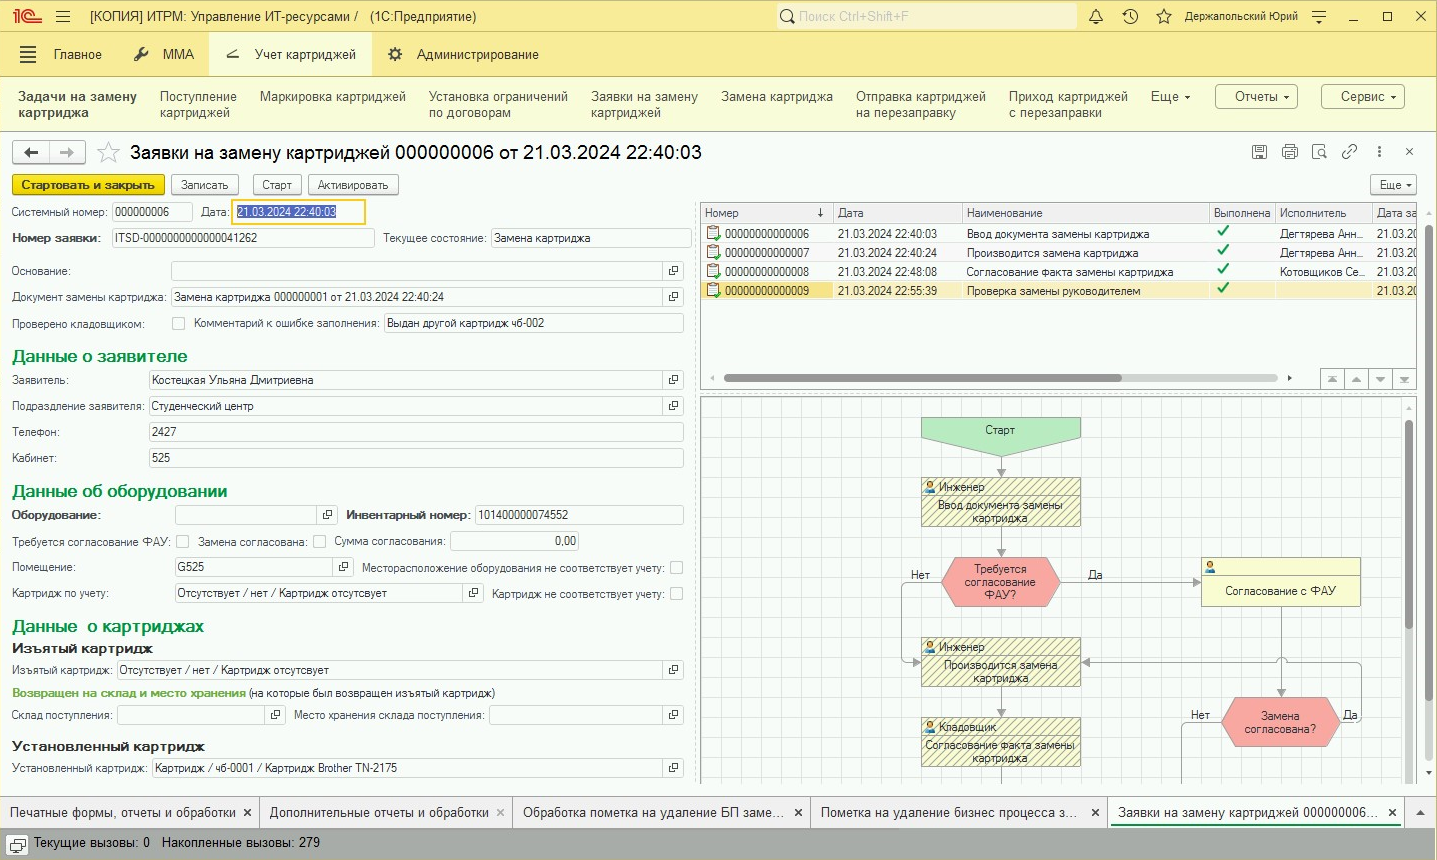
\includegraphics[width=14cm]{pictures/process.png}
    %     % \caption{}  \label{pic_label}
    % \end{figure}

